\section{Results}

\subsection{The corpora overlap far more than exact matching shows}

Table~\ref{tab:overlap} and Fig.~\ref{fig:overlap} show the overlap. Compared
exactly as a model reads them, SpamAssassin and Kaggle share only 2 emails.
With whitespace removed they share 3{,}850, and with near-duplicate matching
5{,}009, which is 86\% of SpamAssassin. The Kaggle set also contains 90\% of
Ling-Spam and 35\% of Enron, and more than half of Kaggle has a copy in Enron.
In other words, the Kaggle ``dataset'' is mostly three older corpora put
together, with formatting changed on the way. Anyone who deduplicates the usual
way, by exact text, would call these corpora independent. The older corpora
also overlap each other: 14\% of SpamAssassin has a near copy in Enron.

CEAS-08, TREC-07, Nazario and E-PhishLLM share almost nothing with any other
source. This gives us a natural control group for the next experiment.

\begin{figure}[t]
\centering
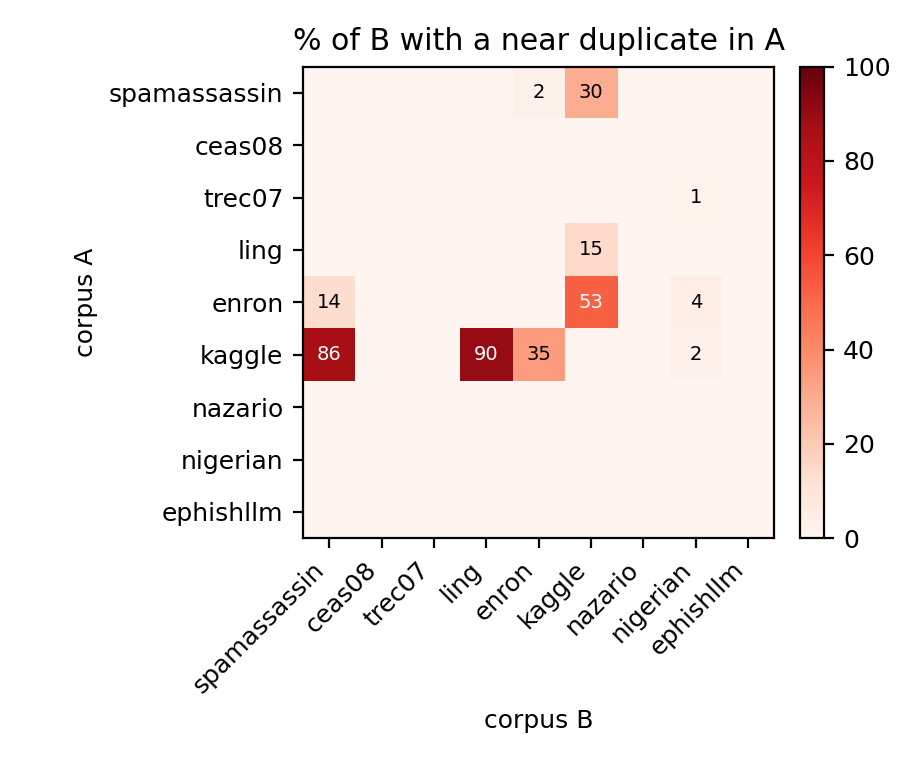
\includegraphics[width=0.88\columnwidth]{overlap_heatmap.png}
\caption{Near-duplicate overlap. Cell $(A,B)$ is the share of corpus $B$ that
has a near duplicate in corpus $A$.}
\label{fig:overlap}
\end{figure}

\begin{table}[t]
\caption{Emails of one corpus found inside another, at three levels of matching. Percentages are of the first corpus.}
\label{tab:overlap}
\centering\footnotesize
\setlength{\tabcolsep}{3pt}
\begin{tabular}{lrrr}
\toprule
Pair & Exact raw & No whitespace & Near duplicate \\
\midrule
SpamAssassin in Kaggle & 2 ($<$0.1\%) & 3,850 (66.3\%) & 5,009 (86.3\%) \\
Ling-Spam in Kaggle & 61 (2.1\%) & 62 (2.2\%) & 2,577 (90.2\%) \\
Enron in Kaggle & 3 ($<$0.1\%) & 187 (0.6\%) & 10,229 (34.5\%) \\
Kaggle in Enron & 3 ($<$0.1\%) & 188 (1.1\%) & 9,212 (52.6\%) \\
SpamAssassin in Enron & 0 (0.0\%) & 122 (2.1\%) & 793 (13.7\%) \\
Nigerian in TREC-07 & 2 ($<$0.1\%) & 2 ($<$0.1\%) & 42 (1.3\%) \\
\bottomrule
\end{tabular}
\end{table}


\subsection{Leaked emails inflate cross-corpus scores}

Table~\ref{tab:pairwise} repeats the one-corpus-to-one-corpus test from our
preliminary work. The Kaggle to SpamAssassin transfer, which looked almost
perfect (F1 0.966), falls to 0.666 once the 2{,}935 Kaggle training emails that
also appear in SpamAssassin are removed. Kaggle to Enron falls from 0.969 to
0.738. The ``good transfer'' was the model recognising emails it had already
seen.

Table~\ref{tab:inflation} shows the same effect in the leave-one-corpus-out
setting. Removing leaked emails lowers Logistic Regression F1 by 11.5 points
on Ling-Spam, 10.0 on SpamAssassin, 5.4 on Enron and 4.8 on Kaggle. For CEAS-08
and TREC-07, which share almost nothing with the other corpora, the change is
0.1 points or less. The inflation appears exactly where the overlap is, which
is strong evidence that leakage, and not some other difference between the
settings, causes it.

Fig.~\ref{fig:incorpus} puts the three settings side by side. The usual
in-corpus split gives 0.93 to 0.99. Honest leave-one-corpus-out testing gives
0.83 to 0.93. The in-corpus number overstates what the model will do on mail
from a new source by 4 to 15 points.

\begin{table}[t]
\caption{Single-corpus transfer with TF-IDF and logistic regression, before and after removing training emails that also appear in the test corpus. The last row is a pair that shares almost nothing.}
\label{tab:pairwise}
\centering\footnotesize
\setlength{\tabcolsep}{3pt}
\begin{tabular}{lrrr}
\toprule
Train $\rightarrow$ test & Removed & Raw F1 & Clean F1 \\
\midrule
Kaggle $\rightarrow$ SpamAssassin & 2,954 & 0.966 & 0.672 \\
Kaggle $\rightarrow$ Enron & 5,511 & 0.969 & 0.661 \\
Kaggle $\rightarrow$ Ling-Spam & 1,450 & 0.979 & 0.837 \\
SpamAssassin $\rightarrow$ Kaggle & 5,032 & 0.766 & 0.590 \\
SpamAssassin $\rightarrow$ Enron & 855 & 0.673 & 0.440 \\
CEAS-08 $\rightarrow$ TREC-07 & 6 & 0.737 & 0.734 \\
\bottomrule
\end{tabular}
\end{table}

\begin{table}[t]
\caption{Leave-one-corpus-out F1 of TF-IDF + Logistic Regression on the full held-out corpus. ``Removed'' is the number of training emails with a near duplicate in the test corpus. $\Delta$ is raw minus clean, in F1 points, for LogReg and Naive Bayes.}
\label{tab:inflation}
\centering\footnotesize
\setlength{\tabcolsep}{3pt}
\begin{tabular}{lrrrrrr}
\toprule
Held out & Removed & In-corpus & Raw & Clean & $\Delta$ LR & $\Delta$ NB \\
\midrule
SpamAssassin & 3,165 & 0.966 & 0.947 & 0.847 & +10.0 & +5.3 \\
Ling-Spam & 1,444 & 0.930 & 0.962 & 0.847 & +11.5 & +4.5 \\
Enron & 6,091 & 0.981 & 0.972 & 0.919 & +5.4 & +5.4 \\
Kaggle & 11,018 & 0.965 & 0.976 & 0.928 & +4.8 & +2.1 \\
CEAS-08 & 13 & 0.986 & 0.833 & 0.832 & +0.1 & +0.0 \\
TREC-07 & 7 & 0.985 & 0.871 & 0.871 & +0.0 & +0.1 \\
\bottomrule
\end{tabular}
\end{table}


\begin{figure}[t]
\centering
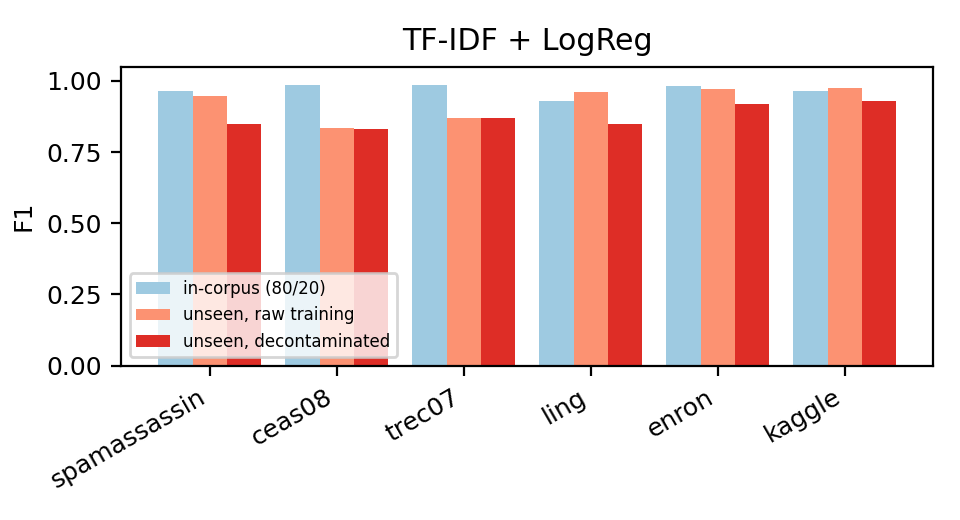
\includegraphics[width=0.95\columnwidth]{incorpus_vs_unseen.png}
\caption{TF-IDF + LogReg F1 per held-out corpus: in-corpus split, unseen
corpus with raw training data, and unseen corpus after decontamination.}
\label{fig:incorpus}
\end{figure}

\subsection{Comparing all models on unseen mail}

Table~\ref{tab:main} is the table our proposal promised: every model on the
same held-out emails, with robustness, AI phishing and cost in one place.
Fig.~\ref{fig:percorpus} breaks the scores down per test set.

\begin{table*}[t]
\caption{Main results. All numbers are on the same fixed evaluation emails. Trained models use decontaminated leave-one-corpus-out data. ``Unseen'' is the mean F1 over the six held-out corpora with a 95\% bootstrap interval, ``Worst'' the lowest of the six. FA is the false alarm rate, the share of legitimate emails flagged as phishing, averaged over the six corpora. AI phishing is F1 on E-PhishLLM. Nazario and Nigerian contain only positives, so we report recall. Cost is the measured OpenRouter charge in USD per 1{,}000 emails.}
\label{tab:main}
\centering\footnotesize
\setlength{\tabcolsep}{4.5pt}
\begin{tabular}{lrrrrrrrrr}
\toprule
Model & In-corpus & Unseen & 95\% CI & Worst & FA (\%) & AI phishing & Nazario rec. & Nigerian rec. & USD/1k \\
\midrule
Qwen-2.5-7B few-shot & -- & 0.937 & 0.925--0.948 & 0.844 & 4.8 & 0.598 & 0.847 & 1.000 & 0.074 \\
Qwen-2.5-7B & -- & 0.928 & 0.915--0.940 & 0.850 & 3.0 & 0.819 & 0.940 & 1.000 & 0.031 \\
TF-IDF + LogReg & 0.969 & 0.901 & 0.886--0.916 & 0.807 & 9.3 & 0.640 & 0.713 & 1.000 & local \\
Llama-3.2-3B few-shot & -- & 0.901 & 0.885--0.915 & 0.848 & 2.7 & 0.438 & 0.680 & 0.993 & 0.037 \\
TF-IDF + NB & 0.929 & 0.895 & 0.879--0.909 & 0.773 & 6.6 & 0.631 & 0.600 & 0.987 & local \\
DistilBERT & 0.975 & 0.891 & 0.875--0.906 & 0.838 & 6.3 & 0.493 & 0.760 & 0.947 & local \\
Gemma-3-12B & -- & 0.882 & 0.866--0.896 & 0.768 & 25.1 & 0.955 & 0.980 & 1.000 & 0.016 \\
Llama-3.1-8B & -- & 0.881 & 0.865--0.896 & 0.779 & 21.4 & 0.817 & 0.973 & 1.000 & 0.011 \\
Llama-3.2-3B & -- & 0.850 & 0.832--0.868 & 0.799 & 5.1 & 0.507 & 0.827 & 1.000 & 0.016 \\
Phi-4-14B & -- & 0.727 & 0.702--0.749 & 0.621 & 27.6 & 0.759 & 0.660 & 0.513 & 0.021 \\
Llama-3.2-1B & -- & 0.623 & 0.597--0.647 & 0.359 & 60.0 & 0.474 & 0.760 & 0.607 & 0.009 \\
\bottomrule
\end{tabular}
\end{table*}


\begin{figure}[t]
\centering
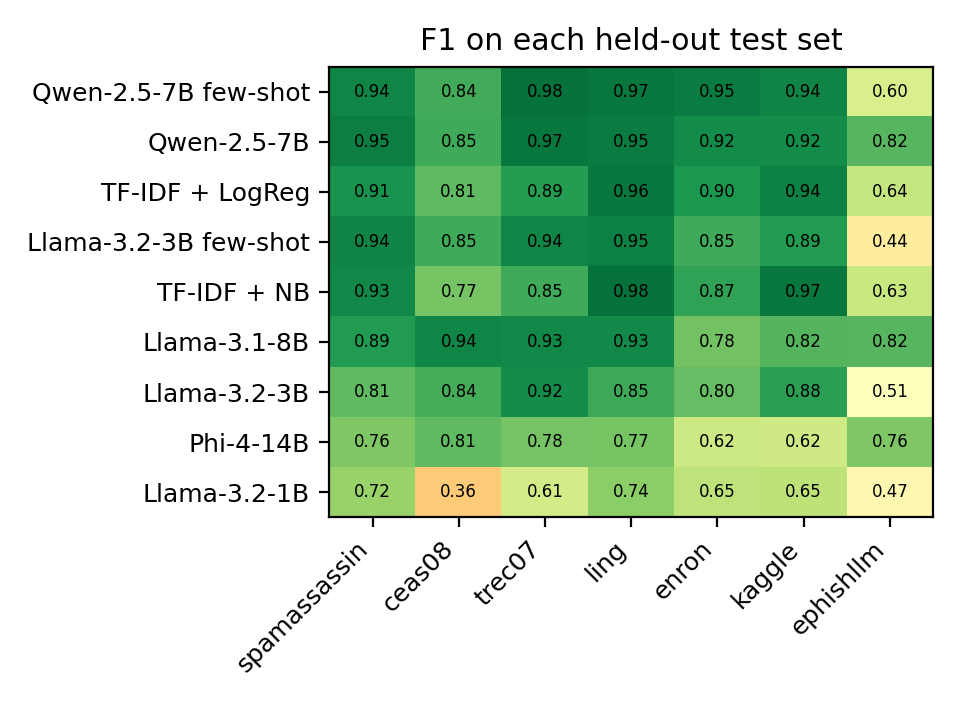
\includegraphics[width=\columnwidth]{per_corpus_f1.png}
\caption{F1 of every model on each held-out test set.}
\label{fig:percorpus}
\end{figure}

\textit{Small LLMs can match or beat trained models on unseen corpora.}
Zero-shot Qwen-2.5-7B reaches a mean F1 of 0.928 on the six held-out
corpora, above TF-IDF + LogReg (0.901) and although Qwen never
saw any of our training data.

\textit{AI-written phishing separates the models.} On E-PhishLLM the trained
models fall to 0.640 (LogReg) and 0.631 (Naive Bayes). They learned
what old spam looks like, and polished GPT-4o-mini phishing does not look like
old spam. Qwen-2.5-7B (0.819) and Llama-3.1-8B (0.817) hold up much better.

\textit{Few-shot examples help on old mail and hurt on new mail.} Four
examples drawn from the other corpora raise Qwen-2.5-7B from 0.928 to
0.937 on the held-out corpora, and Llama-3.2-3B from 0.850 to
0.901. The same examples lower AI-phishing F1 from 0.819 to 0.598
for Qwen and from 0.507 to 0.438 for Llama. The examples come from old
corpora, and they seem to anchor the model to what phishing looked like in
2002 to 2008. Few-shot also more than doubles the cost, because the prompt is
longer.

\textit{Bigger is not automatically better.} Phi-4 (14B) has a lower mean F1
(0.727) than the 3B and 8B Llama models. In 37\% of emails it ignored the
instruction to answer in one word and started an explanation (``As a large
language model\ldots'', ``Based on the content\ldots''), so no verdict fit in the
output.  Llama-3.2-1B is too weak for the task (0.623, with a
worst-corpus F1 of 0.359).

\subsection{Cost}

The measured cost of zero-shot classification ranges from 0.009 to
0.031 US dollars per 1{,}000 emails (Fig.~\ref{fig:cost}). Qwen-2.5-7B
costs 0.031 dollars per 1{,}000 emails, so screening 100{,}000 emails a month
would cost about 3.07 dollars. TF-IDF needs about 0.25 CPU seconds per
1{,}000 emails and no API. DistilBERT needs 0 minutes of laptop GPU time
per training fold and 0 seconds per 1{,}000 emails. The whole study,
18{,}000 LLM calls including discarded trials, cost 0.50 US dollars.

\begin{figure}[t]
\centering
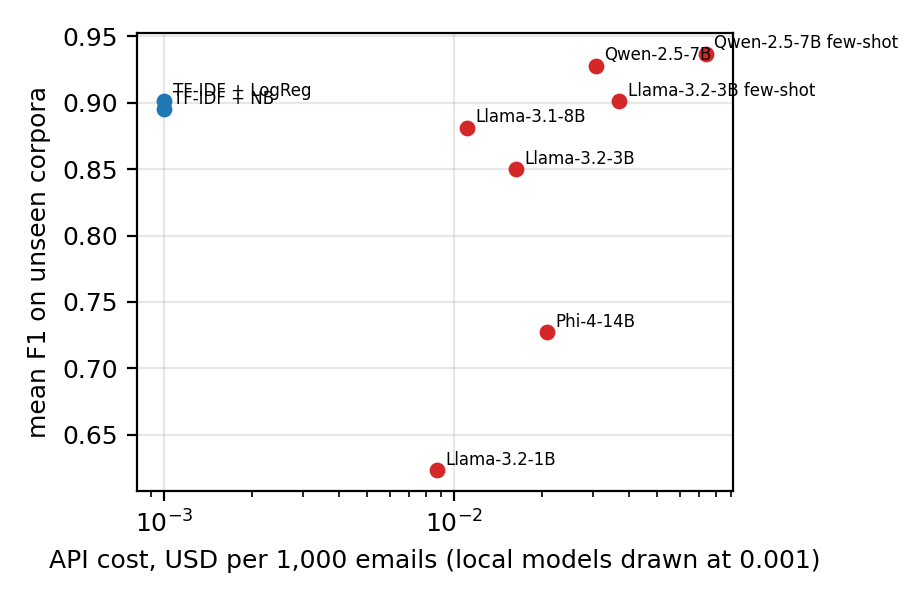
\includegraphics[width=\columnwidth]{f1_vs_cost.png}
\caption{Mean F1 on unseen corpora against measured API cost. Local models
have no API cost and are drawn at 0.001.}
\label{fig:cost}
\end{figure}
